\documentclass[11pt]{article}
\usepackage[margin=1in]{geometry}
\usepackage{amsmath,amssymb,amsthm,bm}
\usepackage{hyperref}
\usepackage{graphicx}
\usepackage{caption}
\usepackage{listings}
\usepackage{xcolor}
\usepackage{float}
\usepackage{placeins}

% Graphics path
\graphicspath{{figures/}}

% Listings style for code
\lstdefinestyle{code}{%
  language=Python,
  basicstyle=\ttfamily\small,
  numbers=left,
  numberstyle=\tiny,
  keywordstyle=\color{blue}\bfseries,
  commentstyle=\color{teal!70!black},
  stringstyle=\color{orange!70!black},
  breaklines=true,
  frame=single,
  rulecolor=\color{black!30},
  tabsize=2,
  showstringspaces=false
}
\lstset{style=code}

\title{Random Forests: Theory and Practice}
\author{}
\date{\today}

\begin{document}
\maketitle

\section{Introduction}
Random forests are ensemble models that aggregate many decision trees trained on bootstrap samples and with randomized feature selection. By averaging (regression) or majority voting (classification), they reduce variance, improve generalization, and retain robustness without extensive preprocessing.

\section{Theory and Formulas}
Random forests combine \emph{bagging} and \emph{feature subsampling}. Let $\{T_b\}_{b=1}^B$ be trees trained on bootstrap samples $\mathcal{D}_b$ and using a random subset of features at each split.
For classification, the prediction is the majority vote
\begin{equation}
\hat{y} = \mathrm{mode}\big( T_1(\mathbf{x}),\dots,T_B(\mathbf{x}) \big),
\end{equation}
and for regression, the average
\begin{equation}
\hat{y} = \frac{1}{B} \sum_{b=1}^B T_b(\mathbf{x}).
\end{equation}
Variance reduces as $B$ increases when individual trees are not perfectly correlated (promoted by feature subsampling). A common choice is $\texttt{max\_features}=\sqrt{p}$ for classification with $p$ features.

\textbf{Out-of-bag (OOB) estimation:} each bootstrap leaves out roughly $\approx 36\%$ of samples. The model's OOB score uses these held-out samples as an internal validation, providing a nearly unbiased generalization estimate without extra cross-validation.

Key hyperparameters: number of trees $B$ (\texttt{n\_estimators}), split feature count (\texttt{max\_features}), tree depth and leaf size (regularization), and bootstrap/OOB settings.

\section{Applications and Tips}
\begin{itemize}
  \item \textbf{Pros:} strong out-of-the-box performance, handles mixed feature types, robust to outliers and monotone transforms, little scaling required.
  \item \textbf{Cons:} larger memory and inference cost than a single tree; less interpretable than a shallow tree.
  \item \textbf{Regularization:} tune \texttt{max\_depth}, \texttt{min\_samples\_leaf}, \texttt{max\_features}; increase \texttt{n\_estimators} until OOB/test metrics stabilize.
  \item \textbf{Diagnostics:} use OOB score, learning curves vs trees, and check feature importances (and, when needed, permutation importance).
  \item \textbf{Preprocessing:} one-hot encode categorical features; no need to standardize numeric features.
\end{itemize}

\section{Python Practice}
Run the script in this chapter directory to generate figures into \texttt{figures/}.
\begin{lstlisting}[style=code,caption={Generate Random Forest figures},label={lst:genfigs_rf}]
python gen_random_forest_figures.py
\end{lstlisting}

% Include the full Python source
\lstinputlisting[style=code,caption={gen\_random\_forest\_figures.py},label={lst:source_rf}]{gen_random_forest_figures.py}

\section{Result}
\begin{figure}[H]
  \centering
  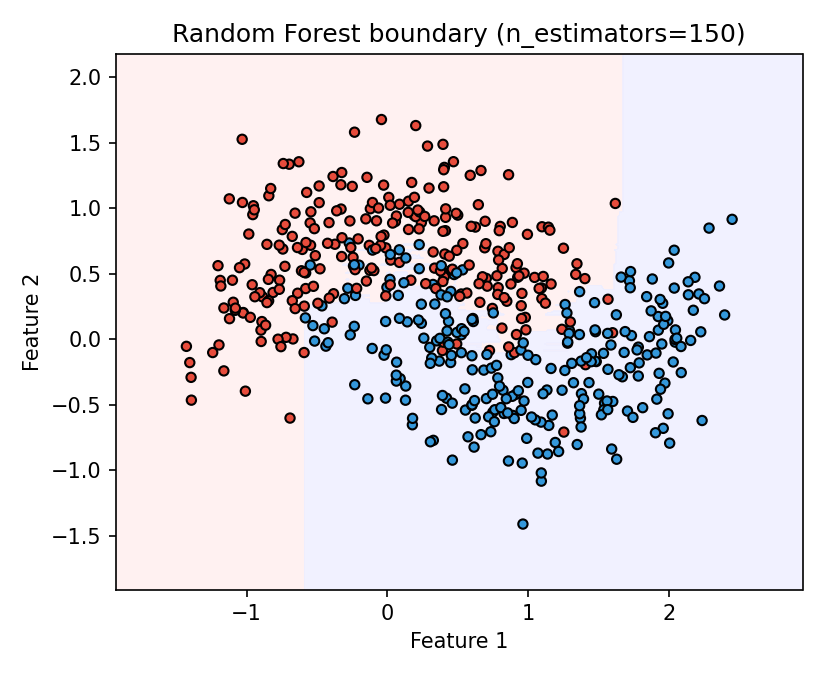
\includegraphics[width=0.9\linewidth]{rf_decision_boundary_2class.png}
  \caption{Random forest decision boundary on a 2-class dataset.}
  \label{fig:rf2}
\end{figure}
\FloatBarrier

\begin{figure}[H]
  \centering
  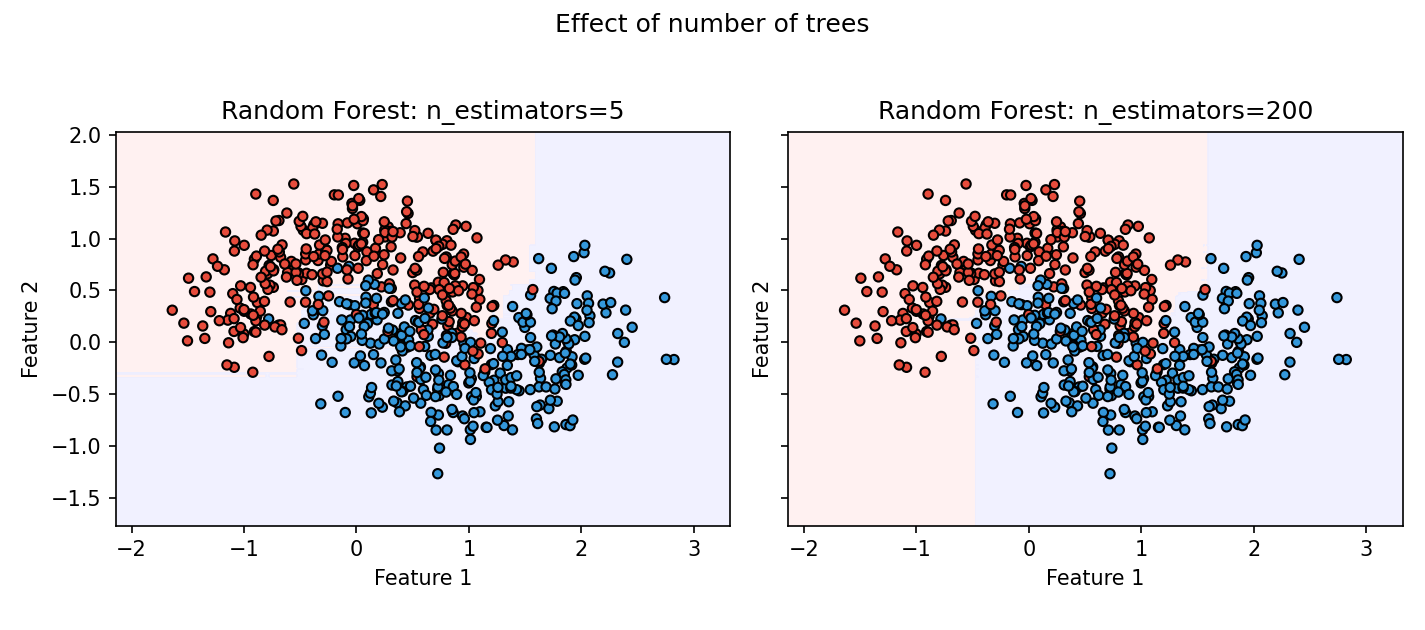
\includegraphics[width=0.95\linewidth]{rf_n_estimators_compare.png}
  \caption{Effect of number of trees: small vs large ensemble.}
  \label{fig:rf_n}
\end{figure}
\FloatBarrier

\begin{figure}[H]
  \centering
  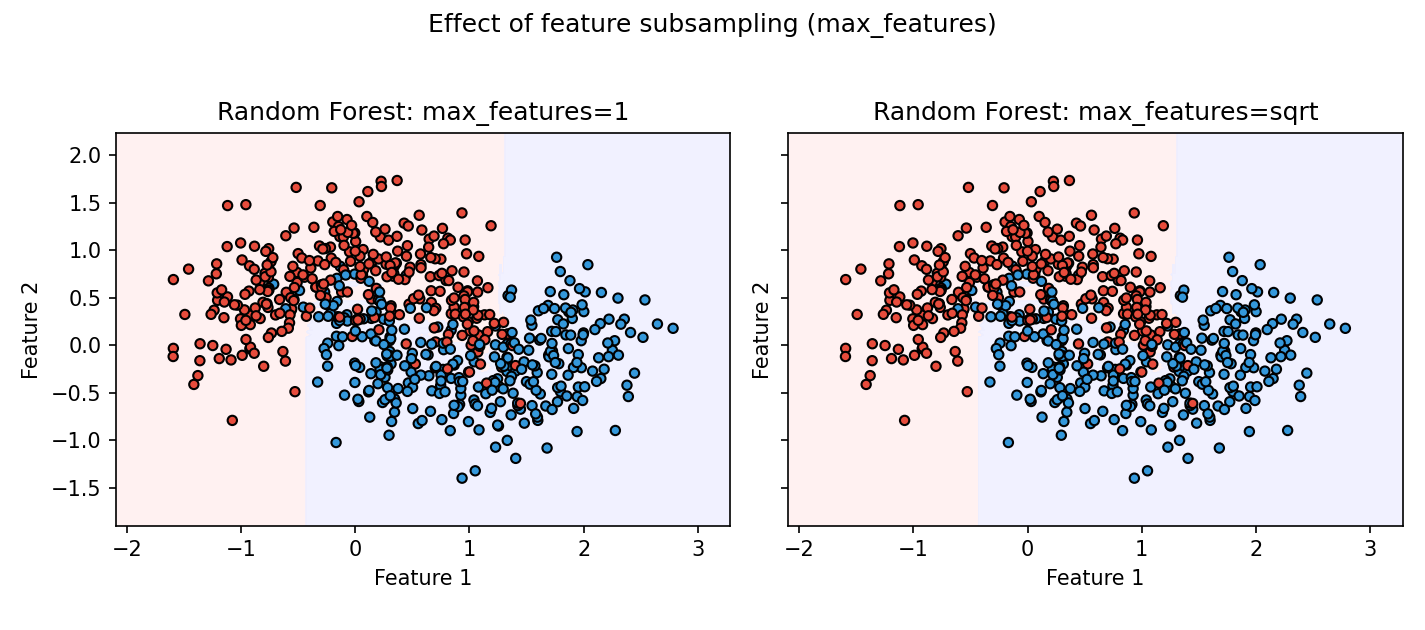
\includegraphics[width=0.95\linewidth]{rf_max_features_compare.png}
  \caption{Decision boundaries with different \texttt{max\_features}.}
  \label{fig:rf_mf}
\end{figure}
\FloatBarrier

\begin{figure}[H]
  \centering
  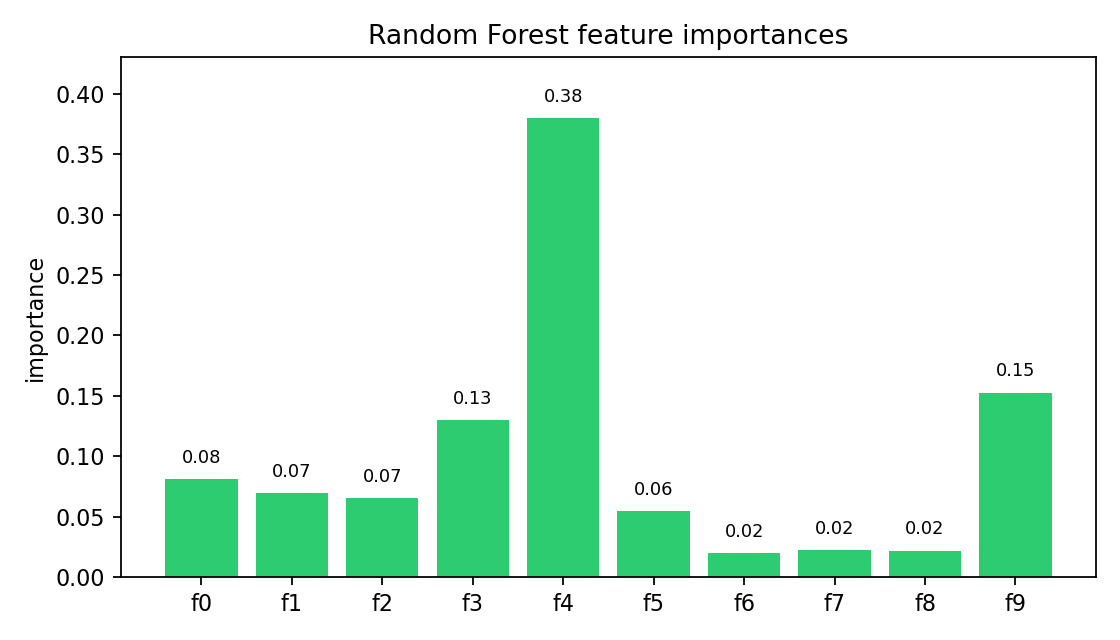
\includegraphics[width=0.85\linewidth]{rf_feature_importances.png}
  \caption{Feature importances from a random forest.}
  \label{fig:rf_fi}
\end{figure}
\FloatBarrier

\begin{figure}[H]
  \centering
  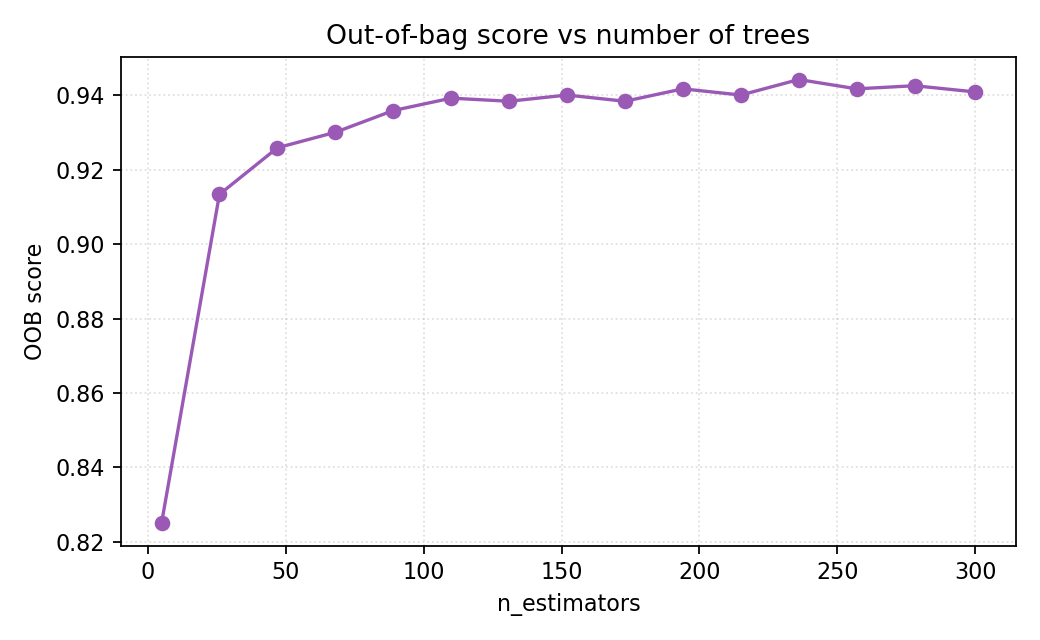
\includegraphics[width=0.85\linewidth]{rf_oob_curve.png}
  \caption{Out-of-bag score vs number of trees.}
  \label{fig:rf_oob}
\end{figure}
\FloatBarrier

\section{Summary}
Random forests provide a strong, reliable baseline for many tasks. They reduce variance through bagging and feature subsampling, offer OOB validation, and yield useful importance measures. Tune tree count and regularization for the best trade-off between accuracy and efficiency.

\end{document}

